% !Mode:: "TeX:UTF-8"
\chapter{相关原理与技术}

\section{程函方程}
程函方程是当使用WKB理论来近似波动方程时在波动传播问题中碰到的非线性偏微分方程。它从电磁学的麦克斯韦尔方程组导出,并在物理 (波动)光学和几何 (射线)光学之间起连接作用。

它的一般形式是:
\begin{equation}
    \label{eikonal_equation_1}
    \left| \nabla u(x) \right| = a(x), x \in \Omega
\end{equation}

约束条件是边界$u(x)$梯度为0。$a(x)$值为正。$\nabla$是梯度,$\left| \right|$是欧几里得范数。这里,右边的$a(x)$是已知的,物理上来说,$u(x)$的求解结果是边界运动到里面某个点$x$所需要的最短时间,此时$a(x)$表示在$x$上花费的时间。

一种快速计算程函方程近似解的方法就是快速行进法。当$a = 1$的特殊情况下,方程的解就是内部点到边界的有符号距离。

在2D情况下,我们求解程函方程,即下面的问题:
\begin{equation*}
    \label{eikonal_equation_2}
    \left\{
    \begin{aligned}
    \left| \nabla u \right| = a & \mbox{on} & \Omega \\
    u = 0 & \mbox{on} &  \partial\Omega
    \end{aligned}
    \right.
\end{equation*}

$\Omega$是平面里面的一个封闭物体。我们离散化变量$x$:$x_{I} = I\Delta x\mbox{其中}I = (I_{1}, I_{2}) \in Z_{2}, \Delta x > 0$。然后将
\begin{equation*}
    \label{eikonal_equation_3}
    \left| \nabla u(x) \right| - a(x) = 0
\end{equation*}

离散化为以下格式:
\begin{equation*}
    \label{scheme}
    S_{I}(\{u_{J}\}_{J \in V(I)}) = 0
\end{equation*}

其中,$V(I) = \{J \in Z^{2}, \left| J - I \right| \leq 1\}$,也就是说$V(I)$是点$I$在平面网格上的相邻5点(看)。于是我们有了
\begin{equation*}
    \label{eikonal_equation_3}
    V(I) = \{I, I^{1, +}, I^{1, -}, I^{2, +}, I^{2, -}\} \mbox{ 其中 } I^{\alpha, \pm}  = I \pm e_{\alpha}, \alpha = 1, 2
\end{equation*}

我们推荐Rouy-Tourin格式
\begin{equation}
    \label{eikonal_equation_3}
    \begin{aligned}
    & -a(x_I) + \sqrt{(\max(0, \frac{u_I - u_{I^{1, -}}}{\Delta x}, \frac{u_I - u_{I^{1, +}}}{\Delta x}))^2 + (\max(0, \frac{u_I - u_{I^{1, -}}}{\Delta x}, \frac{u_I - u_{I^{1, +}}}{\Delta x}))^2} \\
    & := S_I(u_I, u_{I^{1, -}}, u_{I^{1, +}}, u_{I^{2, -}}, u_{I^{2, +}}) := S_I[u]
    \end{aligned}
\end{equation}

\section{快速行进法}
\subsection{数学证明}
快速行进法(Fast Marching Method, FMM)是由Sethian在1996年提出的,用来求解从已知边界向内部演化的过程。它以某种方式记录了物体边界向前行进的信息。
\begin{figure}[h!]
    \centering
    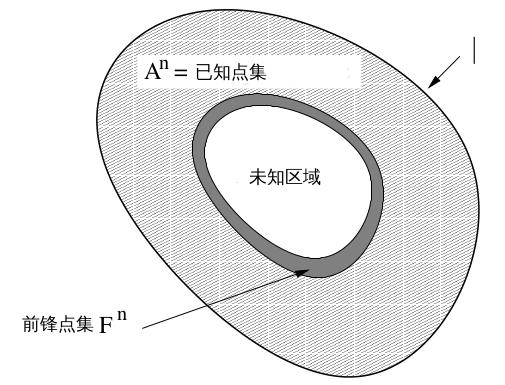
\includegraphics[width=300bp]{figure/sets_fmm.png}
    \caption{FMM的各个集合:已知点集$A^n$,前锋点集$F^n$和未知区域}
    \label{fig-sets_fmm}
\end{figure}

首先我们定义一个递增时间序列$(t_{n})_{n}$,其中$t_{0} = 0$,一个递增集合序列$(A^{n})_{n}$和一个非递增函数序列$(u^{n})_{n}$,其中,每一个$Z^{2}$网格上的点$I$都对应定义$u^{n} = (u^{n}_{I})_{I}$。$u^n$在$A^n$上面计算出来的值就是程函方程里$u$的解。这也是为什么$A^n$被称为已知点集,因为$u^n$与$A^n$外面的点没有关系,我们设置
\begin{equation*}
    \label{far_region}
    u^n_I = +\infty \mbox{当} I \in Z^2 \setminus A^n
\end{equation*}

另一方面,$t_n$的值是
\begin{equation*}
    \label{tn_in_fn}
    u^n_I = t_n \mbox{当} I \in A^2 \setminus A^{n-1}
\end{equation*}

即$t_n$是已知点集$A^n$中相对于$A^n$新增的点的一般值。

看图很容易就能想到,前锋点集$F^n$就是已知点集$A^n$的离散边界,就是说
\begin{equation*}
    \label{fn_1}
    F^n = \{ I \in Z^2 \setminus A^n, \mbox{所以} V(I)\cap A^n \neq \textrm \O \}
\end{equation*}

为了更方便的应用到FMM算法里面,我们改写上式为
\begin{equation*}
    \label{fn_2}
    F^n = ( \underset{I \in A^n}{\cup}V(I)) \setminus A^n
\end{equation*}

前锋点集$F^n$是在$A^n$外面,离$A^n$很近的一组网格点。所以我们又称前锋点集为“窄带”。我们将要在这个点集里面为$A^{n+1} \setminus A^n$寻找新的点,即
\begin{equation*}
    \label{fn_3}
    A^{n+1} \setminus A^n \subset F^n
\end{equation*}
$A^n \cup F^n$的补集就被成为未知区域,因为这些点在第$n$步到第$n+1$步都不会被用到。

重要的是确定$F^n$里面哪些点可以被包含到$A^{n+1} \setminus A^n$里面。为了达到这个目的,我们先对每个前锋点集$F^n$里面的点$I$计算一个值$\widetilde{u}^n_I$。这个值是$u_I$的一个候选值(可能比$u_I$更大)。在这些值里面,我们只取最小的那个值
\begin{equation*}
    \label{tn+1}
    t_{n+1} = \underset{I \in F^n}{\min}\widetilde{u}^n_I
\end{equation*}
这些点就是新的已知点。也就是说
\begin{equation*}
    \label{tn+1}
    A^{n+1} \setminus A^n = \{ I \in F^n, \widetilde{u}^n_I = t_{n+1}\}
\end{equation*}
这恰好就解释了函数$u$的值就是从$\Omega$边界到达点$x_I$所花费的最短时间。我们定义新的$u^{n+1}$
\begin{equation*}
    \label{un+1}
    u^{n+1}_I = \left\{
    \begin{aligned}
    & t_{n+1} & I \in A^{n+1} \setminus A^n \\
    & u^n_I & \mbox{其他}
    \end{aligned}
    \right.
\end{equation*}

那么怎么计算这个$\widetilde{u}^n_I$的值呢?
对于给定的函数$u^n$,我们只需要找到下面方程的解$\widetilde{u}^n_I$。
\begin{equation}
    \label{solve_un}
    S_I(\widetilde{u}^n_I, \{u^n_J\}_{J \in V(I) \setminus \{I\}}) = 0
\end{equation}
要注意的是,如果$I$的相邻点$J$的值$u^n_J = +\infty$,这个点在计算的时候是不使用的,因为这种点在已知点集的补集里面,它们没有携带任何信息。我们只取在$A^n$里面的$J$点。例如图片\ref{closer_points},$A, B$在$A^n$里面,$C, D$不在$A^n$里面($C$在前锋上,$D$在未知区域)。所以$C, D$在计算$\widetilde{u}^n_I$是不会用到的。只有$J = A, B$对应的$u^n_J = u_J$会被用来计算$\widetilde{u}^n_I$。
\begin{figure}[h!]
    \centering
    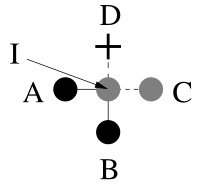
\includegraphics[width=150bp]{figure/closer_points.png}
    \caption{$I$点相邻点}
    \label{closer_points}
\end{figure}

接下来我们看一下快速行进法的算法描述:

初始化
\begin{equation*}
    \label{fmm_init}
    \left\{
    \begin{aligned}
    & t_0 & = & 0 \\
    & A^0 & = & \{I \in Z^2, x_I \notin \Omega\} \\
    & u^0_I & = & \left\{
        \begin{aligned}
        & 0 & I \in A^0 \\
        & +\infty & I \notin A^0
        \end{aligned}
        \right.
    \end{aligned}
    \right.
\end{equation*}

从第$n$步到第$n+1$步,我们假设$t_n, A^n, u^n$都已知。

首先,我们计算时间的候选值$\widetilde{u}^n_I$,对于每一个$I \in F^n$,找到$\widetilde{u}^n_I$的唯一解:
\begin{equation*}
    \label{uI_unique}
    0 = S_I(\widetilde{u}^n_I, \{u^n_J\}_{J \in V^*(I)}), \mbox{其中} V^*(I) = V(I) \setminus \{I\}
\end{equation*}

然后,取最小的候选值。
\begin{equation*}
    \label{min_tn+1}
    t_{n+1} = \underset{I \in F^n}{\inf} \widetilde{u}^n_I
\end{equation*}

最后,更新点集和各个函数值。新的已知点集为
\begin{equation*}
    \label{new_an+1}
    NA^{n+1} = \{I \in F^n, \widetilde{u}^n_I = t_n\}
\end{equation*}
可得
\begin{equation*}
    \label{new_values}
    \left\{
    \begin{aligned}
    & t_{n+1},\\
    & A^{n+1} & = & A^n \cup NA^{n+1}, \\
    & u^{n+1}_I & = & \left\{
        \begin{aligned}
        & t_{n+1} & I \in NA^n \\
        & u^n_I & \mbox{其他}
        \end{aligned}
        \right.
    \end{aligned}
    \right.
\end{equation*}

算法结束。

\subsection{伪代码}
\label{pseudocode}
这里我们考虑方程\ref{eikonal_equation_1}的特殊情况:$a = 1$,即
\begin{equation}
    \label{special_eikonal_equation}
    \left| \nabla u(x) \right| = 1
\end{equation}
其中$u = 0$在物体的边界上。这个时候的$u$是物体边缘到内部点的距离的很好的近似。
快速行进法在算法上很容易实现,对于每一个2D网格点或者坐标为$(i, j)$的像素点,我们存储它的距离变换的浮点数值$T_{ij}$和一个标志$f_{ij}$。这个标志可能有三个值:
\begin{itemize}
\item BAND: 表示点属于当前的前锋点集或者说窄带($F^n$),他的$T$值依然在变化中。
\item INSIDE: 表示点在移动前锋内部的未知点集,它的$T$值目前未知。
\item KNOWN: 表示点在移动前锋后面(已知点集$A^n$),它的$T$值已知。
\end{itemize}

初始化如代码\ref{fmm_init_code}所示,MAX\_VALUE表示比任何可能的$T$都要大的值,比如说$10^6$。
\begin{lstlisting}[
    language={C},
    caption={快速行进法初始化代码},
    label={fmm_init_code},
]
for all points (i,j)
{
    if ((i,j) on initial boundary)
    {
        f(i,j)=BAND; T(i,j)=0;
        add (i,j) to NarrowBand;
    }
    else if ((i,j) inside boundary)
    {
        f(i,j)=INSIDE; T(i,j)=MAX_VALUE;
    }
    else /* (i,j) outside boundary */
    {
        f(i,j)=KNOWN; T(i,j)=0;
  }
}
\end{lstlisting}

演化时,我们将方程\ref{special_eikonal_equation}离散近似为:
\begin{equation}
    \label{discretized_eikonal_equation}
    \max(D^{-x}T, -D^{+x}T, 0)^2 + \max(D^{-y}T, -D^{+y}T, 0)^2 = 1
\end{equation}
其中$D^{-x}T(i, j) = T(i, j) - T(i - 1, j)$,并且$D^{+x}T(i, j) = T(i + 1, j) - T(i, j)$,$y$轴方向类似。方程\ref{special_eikonal_equation}可以由循环在每个网格点求解方程\ref{discretized_eikonal_equation}得到结果,对于$N$个网格点时间复杂度是$O(N^2)$。如代码\ref{fmm_iteration_code}所示。
\begin{lstlisting}[
    language={C},
    caption={快速行进法迭代代码},
    label={fmm_iteration_code},
]
while (NarrowBand not empty)
{
    P(i,j)=head(NarrowBand); 						/* STEP 1 */
    remove P from NarrowBand;
    f(i,j)=KNOWN;
    for point (k,l) in {(i−1,j),(i,j−1),(i+1,j),(i,j+1)}
        if (f(k,l)!=KNOWN)
        {
            if (f(k,l)==INSIDE) f(k,l)=BAND; 	    /* STEP 2 */
            sol=MAX_VALUE; 							/* STEP 3 */
            solve(k−1,l,k,l−1,sol);
            solve(k+1,l,k,l−1,sol);
            solve(k−1,l,k,l+1,sol);
            solve(k+1,l,k,l+1,sol);
            T(k,l)=sol;
            insert (k,l) in NarrowBand; 			/* STEP 4 */
        }
}

solve(int i1,int j1,int i2,int j2,float& sol)
{
    float r,s;
    if (f(i1,j1)==KNOWN)
        if (f(i2,j2)==KNOWN)
        {
            r = sqrt((2−(T(i1,j1)−T(i2,j2))*(T(i1,j1)−T(i2,j2)));
            s = (T(i1,j1)+T(i2,j2)−r)/2;
            if (s>=T(i1,j1) && s>=T(i2,j2)) sol=min(sol,s);
            else
            {
                s += r;
                if (s>=T(i1,j1) && s>=T(i2,j2)) sol=min(sol,s);
            }
        }
        else sol=min(sol,1+T(i1,j1));
    else if (f(i2,j2)==KNOWN) sol=min(sol,1+T(i1,j2));
}
\end{lstlisting}

\section{增强快速行进法}
快速行进法计算的是内部点到边界的距离,这里介绍一下增强的快速行进法用来产生骨架。图表\ref{skel_overview}概述了算法应用到一个锯齿状矩形的整个过程。
\begin{figure}[h!]
    \centering
    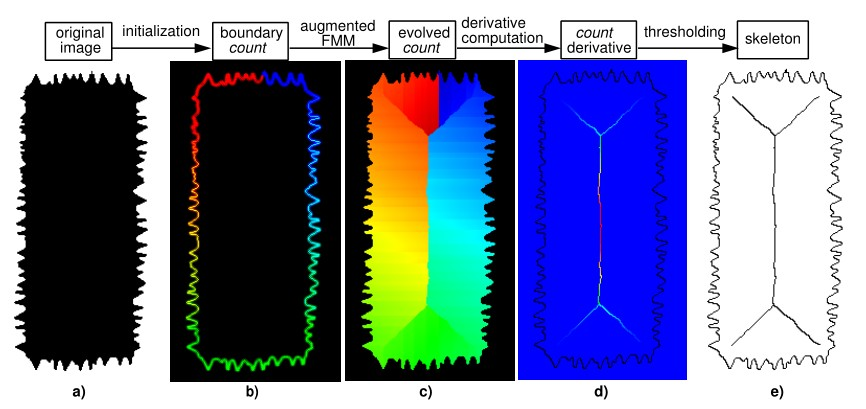
\includegraphics[height=200bp]{figure/skel_overview.png}
    \caption{骨架提取算法预览}
    \label{skel_overview}
\end{figure}
很容易想到骨架点总是由紧凑的边界段在前锋行进时重合产生的。这个方法的重点就在于确定每一个行进前锋上的点是由边界上哪个点得来,为了实现这个目的,我们为每个网格点新增了一个实数属性$U$。初始化时,我们选取任意一个边界点,设置$U=0$,从这个点开始,我们为每个边界点设置一个单调递增的$U$值,这个$U$值等于这个点沿边界到初始点的长度。所以$U$是边界上两点沿边界的距离参数化的结果。有个例外就是$U$在各自的连通边界上开始演化,这个我们后面再讲。

初始化后,$U$和$T$一起演化(图片\ref{skel_overview})。我们在步骤2的演化代码(代码\ref{fmm_iteration_code})中加了一些语句来实现这步,如代码\ref{afmm_step2}。
\begin{lstlisting}[
    language={C},
    caption={增强快速行进法增加的代码},
    label={afmm_step2},
]
… original FMM code …
If (f(k, l) == INSIDE)	/* STEP 2*/
{
	F(k, l) = BAND;
	a = average of U over KNOWN neighbors of (k, l);
	m = min of U over KNOWN neighbors of (k, l);
	M = max if U over KNOWN neighbors of (k, l);
	If (M – m < 2) U(k, l) = a; else U(k, l) = U(i, j);
}
… original FMM code
\end{lstlisting}

在$U$的演化过程中,将初始边界内部的像素点的$U$值标记为到达这个点的边界点的U值。对于初始边界像素点中间的边界点我们使用平均法进行插值计算$U$值。这在边界段是凹面,向前行进边界会变长的时候发生。然而,如果当前点的$U$值相差大于2,这意味着他们在边界上的原点不是相邻点,因为边界上相邻点之间的距离最大为$\sqrt2$,如图\ref{neighbor_distance}里面斜对角的两个点。
\begin{figure}[h!]
    \centering
    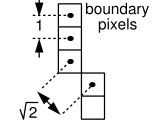
\includegraphics[height=70bp]{figure/neighbor_distance.png}
    \caption{相邻点距离}
    \label{neighbor_distance}
\end{figure}
以上情况发生在凸的边界段,它们在前锋行进的时候会发生重合。这时,我们就发现了一个骨架点,不用计算$U$的平均值,我们只需要选取其中一个相邻点的$U$值继续演化下去即可。图片\ref{afmm_details}有增强快速行进法的举例说明,例子中计算了一个矩形的骨架。
\begin{figure}[h!]
    \centering
    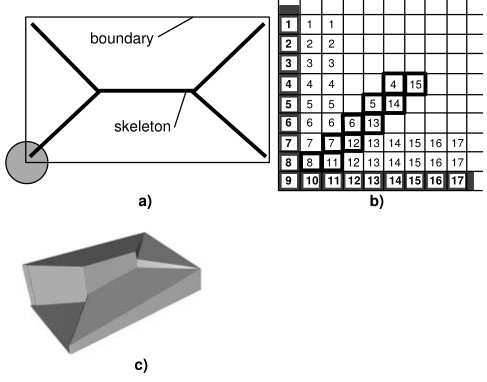
\includegraphics[height=180bp]{figure/afmm_details.png}
    \caption{增强快速行进法的执行细节}
    \label{afmm_details}
\end{figure}
图中b部分展示了前三个带有$U$值的窄带,他们和矩形的边是平行的,这时没有骨架分支出现,前锋上的U值和边界上是一样的,也就是说,相邻点之间$U$差值为1。然而,在骨架分支上,这个差值离边界越远会变得越大,图中c的3D图像表明了这点。

在前面提到过,$U$在上递增地进行参数化时,这个起点位置的$U$不再是边界上两点沿边界的距离参数化的结果,他与该边界上最大的$U$是挨着的,但是$U$的差值却是最大的。对于图片\ref{special_points},有3个这样的点,相应就有3个不连通的边界段。图片\ref{special_points}展示了初始的$U$值,和数字编号,并使用了彩色进行标注(蓝色代表低值,红色代表高值,打印版可能只剩下灰度)。根据上面说的,这个$U$域有3个假的不连续的地方,如图片中的c。骨架(图中的d)就会得到3个假分支,就是那3个垂直指向边界的分支。
\begin{figure}[h!]
    \centering
    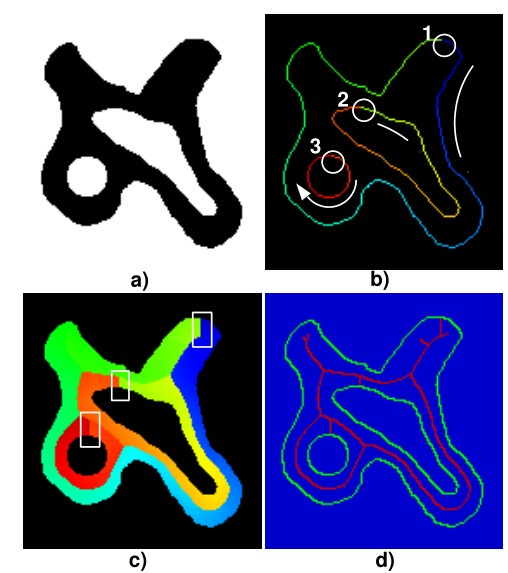
\includegraphics[height=250bp]{figure/special_points.png}
    \caption{特殊点的处理:原始物体(a),初始$U$(b),计算出来的$U$(c),骨架(d)}
    \label{special_points}
\end{figure}

移除这些假分支很容易,我们执行增强快速行进法两次,并且从不同的边界位置开始初始化$U$值。比如说,最小的y坐标值对应最大的y坐标值的点。下一步,我们对两个骨架求交集来移除假分支。这种方法在我们所有的测试用例中都生成了正确的骨架。

\section{3D中心路径提取}
\label{afmm-3D}
我们很希望上一节介绍的增强快速行进法方法可以推广到三维,因为3D中心路径提取也是一个十分诱人的应用场景,3D中心路径可以用来3D路径规划和导航,目标识别和物体简化等。但是由于我们使用的方法依赖于2D物体边界点之间沿边界的距离,而2D曲线和3D曲面的拓扑属性和排序方法在本质上是不同的。所以很不幸的是,这个方法不能直接推广到3D。

然而,我们可以通过另外的方法将这个2D骨架提取算法用于计算3D中心路径。我们知道3D中心路径是一条曲线,它是由3D物体内部容纳下的最大球球心的路径,即如果一个点属于中心路径,那么他是离物体边界最远的点,这和2D的情况是一致的。

我们可以这样计算3D中心路径。首先,我们使用增强快速行进法计算3D体数据每个与坐标轴平行的2D切片的2D骨架。这将生成3个2D骨架束,或者说3个体数据,对应3个切片方向,我们称之为X,Y,Z骨架。接下来,我们对这些体数据逐个像素取交集,保存下初始3D物体的中心线。
显然,交集中的体像素属于3个坐标轴对应的2D骨架。用这3个正交的切片平面来说,这些像素点就是离边界距离最远的点。这种方法是对一般情况的简化,一般方法里我们需要计算点到边界在任意切分平面的距离,这里我们使用了3个正交的圆而不是球。然而,这种方法对于通常需要计算的典型的绳状物体来说已经足够的近似了。

但是这个方法一个缺点就是,就算2D的骨架是连通的,3D中心线却不能保证也连通,尤其在初始体数据分辨率很低的时候。
